\chapter{Introduzione}
La sindrome del \textit{BlueBaby} ri riferisce ad un insieme variegato di condizioni anomale e a volte patologiche che si manifestano nella colorazione cianotica della pelle del neonato.
L'obiettivo principale dei medici è quello di trovale quale delle patologie che possono portare al colorito blu della pelle sia presente nel bambino, al fine di intervenire repentinamente e contenere così i rischi. Per fare ciò, i medici hanno a disposizioni una serie di esami clinici da compiere, che permettono di rilevare i sintomi tipici di alcune malattie che sono anche causa della sindrome in questione. Analizzando questi risultati, i medici sono in grado di restringere le possibili malattie che affliggono il neonato, individuando così la causa più probabile della colorazione anomala della pelle.

Nel nostro caso, alcuni ricercatori hanno lavorato a stretto contatto con medici ed esperti e sono riusciti a produrre una rappresentazione delle rete di dipendenza del fenomeno (\textit{Spiegelhalter, David J., et al. "Bayesian analysis in expert systems." Statistical science 8.3 (1993): 219-247.}). La rete prodotta, riportata in Figura \ref{fig:paperstructure}, contiene una serie di sintomi, esami e dati sul paziente che permettono di modificare la probabilità che una malattia sia presente nell'infante. L'ipotesi a priori assunta è che non coesista più di una causa contemporaneamente per la sindrome studiata. Possiamo vedere come i nodi della rete si dispongano secondo una struttura ad albero; in particolare, i figli del nodo \textit{Disease} sono situazioni patologiche manifestate in alcune delle malattie che possono causare la sindrome in analisi. I figli di questi nodi sono o nuove situazioni patologiche causalmente collegate alle precedenti, o esami che permettono di accertarne la presenza.
 
 \begin{figure}
 	\centering
 	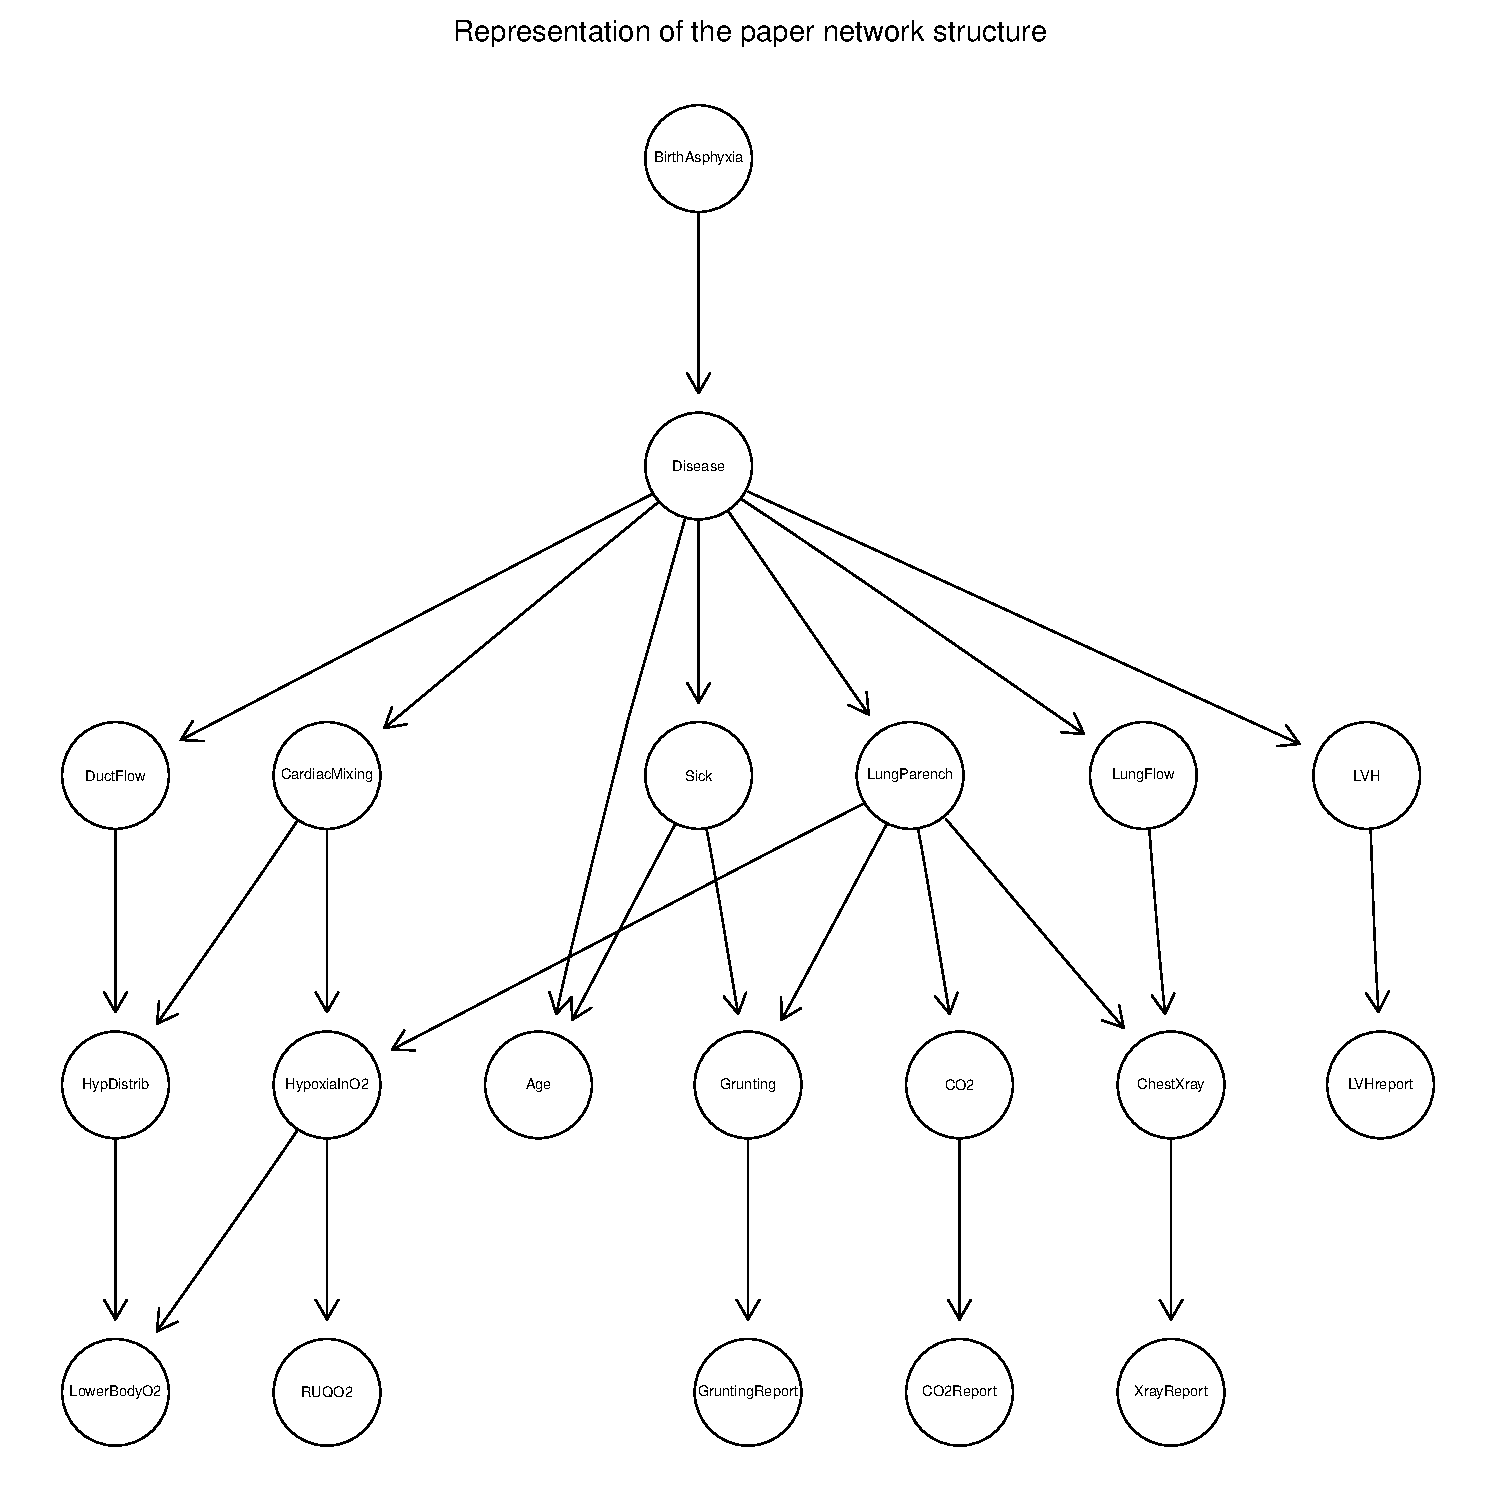
\includegraphics[width=1\linewidth]{images/paper_structure}
 	\caption{Rappresentazione della rete prodotta dai ricercatori, in collaborazione con medici ed esperti. Ogni nodo rappresenta un sintomo, un esame o un dato del paziente.}
 	\label{fig:paperstructure}
 \end{figure}

\section{Obiettivi}
Nel nostro lavoro, abbiamo voluto studiare se fosse possibile inferire la struttura della rete a partire da un dataset contenete evidenze dei nodi della rete in casi accertati della sindrome del \textit{BlueBaby}. Cercheremo poi di capire se vi siano dei nodi che sono condizionalmente indipendenti da altri nodi data l'evidenza di un insieme di variabili, in modo da consentire la riduzione del numero di esami necessari al fine di ottenere una diagnosi accurata. Vaglieremo infine la possibilità di utilizzare la rete invertendo le relazioni da causalità, analizzando i risultati ottenuti e comparandoli quelli della rete proposta.